%%%%%%%%%%%%%%%%%%%% book.tex %%%%%%%%%%%%%%%%%%%%%%%%%%%%%
%
% sample root file for the chapters of your "monograph"
%
% Use this file as a template for your own input.
%
%%%%%%%%%%%%%%%% Springer-Verlag %%%%%%%%%%%%%%%%%%%%%%%%%%


% RECOMMENDED %%%%%%%%%%%%%%%%%%%%%%%%%%%%%%%%%%%%%%%%%%%%%%%%%%%
\documentclass[graybox,envcountchap,sectrefs]{style/svmono}

% choose options for [] as required from the list
% in the Reference Guide

%\usepackage{mathptmx}
%\usepackage{helvet}
%\usepackage{courier}
%
\usepackage{kotex}

\usepackage{setspace}

\usepackage{type1cm}         

\usepackage{makeidx}         % allows index generation
\usepackage{graphicx}        % standard LaTeX graphics tool
\usepackage{float}
                             % when including figure files
\usepackage{multicol}        % used for the two-column index
\usepackage[bottom]{footmisc}% places footnotes at page bottom

\usepackage{multirow}

\usepackage{physics}
\usepackage{newtxtext}       % 
%\usepackage{newtxmath}       % selects Times Roman as basic font
\usepackage[subscriptcorrection,mtpcal,mtphrd,nofontinfo]{mtpro2}

% see the list of further useful packages
% in the Reference Guide

\makeindex             % used for the subject index
                       % please use the style svind.ist with
                       % your makeindex program

%%%%%%%%%%%%%%%%%%%%%%%%%%%%%%%%%%%%%%%%%%%%%%%%%%%%%%%%%%%%%%%%%%%%%

\graphicspath{{./}{images/}}

\begin{document}

\author{R. Shankar}
\title{Principles of Quantum Mechanics}
\subtitle{second edition}
\maketitle

\frontmatter%%%%%%%%%%%%%%%%%%%%%%%%%%%%%%%%%%%%%%%%%%%%%%%%%%%%%%
\setstretch{1.4}

%
%%%%%%%%%%%%%%%%%%%%%%% dedic.tex %%%%%%%%%%%%%%%%%%%%%%%%%%%%%%%%%
%
% sample dedication
%
% Use this file as a template for your own input.
%
%%%%%%%%%%%%%%%%%%%%%%%% Springer %%%%%%%%%%%%%%%%%%%%%%%%%%

\begin{dedication}
Use the template \emph{dedic.tex} together with the Springer document class SVMono for monograph-type books or SVMult for contributed volumes to style a quotation or a dedication\index{dedication} at the very beginning of your book
\end{dedication}





%%%%%%%%%%%%%%%%%%%%%%%foreword.tex%%%%%%%%%%%%%%%%%%%%%%%%%%%%%%%%%
% sample foreword
%
% Use this file as a template for your own input.
%
%%%%%%%%%%%%%%%%%%%%%%%% Springer %%%%%%%%%%%%%%%%%%%%%%%%%%

\foreword

%% Please have the foreword written here
Use the template \textit{foreword.tex} together with the document class SVMono (monograph-type books) or SVMult (edited books) to style your foreword\index{foreword}. 

The foreword covers introductory remarks preceding the text of a book that are written by a \textit{person other than the author or editor} of the book. If applicable, the foreword precedes the preface which is written by the author or editor of the book.


\vspace{\baselineskip}
\begin{flushright}\noindent
Place, month year\hfill {\it Firstname  Surname}\\
\end{flushright}



%%%%%%%%%%%%%%%%%%%%%%%preface.tex%%%%%%%%%%%%%%%%%%%%%%%%%%%%%%%%%%%%%%%%%
% sample preface
%
% Use this file as a template for your own input.
%
%%%%%%%%%%%%%%%%%%%%%%%% Springer %%%%%%%%%%%%%%%%%%%%%%%%%%

\preface

%% Please write your preface here
Use the template \emph{preface.tex} together with the document class SVMono (monograph-type books) or SVMult (edited books) to style your preface.

A preface\index{preface} is a book's preliminary statement, usually written by the \textit{author or editor} of a work, which states its origin, scope, purpose, plan, and intended audience, and which sometimes includes afterthoughts and acknowledgments of assistance. 

When written by a person other than the author, it is called a foreword. The preface or foreword is distinct from the introduction, which deals with the subject of the work.

Customarily \textit{acknowledgments} are included as last part of the preface.
 

\vspace{\baselineskip}
\begin{flushright}\noindent
Place(s),\hfill {\it Firstname  Surname}\\
month year\hfill {\it Firstname  Surname}\\
\end{flushright}



%%%%%%%%%%%%%%%%%%%%%%%acknow.tex%%%%%%%%%%%%%%%%%%%%%%%%%%%%%%%%%%%%%%%%%
% sample acknowledgement chapter
%
% Use this file as a template for your own input.
%
%%%%%%%%%%%%%%%%%%%%%%%% Springer %%%%%%%%%%%%%%%%%%%%%%%%%%

\extrachap{Acknowledgements}

Use the template \emph{acknow.tex} together with the document class SVMono (monograph-type books) or SVMult (edited books) if you prefer to set your acknowledgement section as a separate chapter instead of including it as last part of your preface.



\tableofcontents

%%%%%%%%%%%%%%%%%%%%%%acronym.tex%%%%%%%%%%%%%%%%%%%%%%%%%%%%%%%%%%%%%%%%%
% sample list of acronyms
%
% Use this file as a template for your own input.
%
%%%%%%%%%%%%%%%%%%%%%%%% Springer %%%%%%%%%%%%%%%%%%%%%%%%%%

\extrachap{Acronyms}

Use the template \emph{acronym.tex} together with the document class SVMono (monograph-type books) or SVMult (edited books) to style your list(s) of abbreviations or symbols.

Lists of abbreviations\index{acronyms, list of}, symbols\index{symbols, list of} and the like are easily formatted with the help of the Springer-enhanced \verb|description| environment.

\begin{description}[CABR]
\item[ABC]{Spelled-out abbreviation and definition}
\item[BABI]{Spelled-out abbreviation and definition}
\item[CABR]{Spelled-out abbreviation and definition}
\end{description}


\mainmatter%%%%%%%%%%%%%%%%%%%%%%%%%%%%%%%%%%%%%%%%%%%%%%%%%%%%%%%
%%%%%%%%%%%%%%%%%%%%%%part.tex%%%%%%%%%%%%%%%%%%%%%%%%%%%%%%%%%%
% 
% sample part title
%
% Use this file as a template for your own input.
%
%%%%%%%%%%%%%%%%%%%%%%%% Springer %%%%%%%%%%%%%%%%%%%%%%%%%%

\begin{partbacktext}
\part{Part Title}
\noindent Use the template \emph{part.tex} together with the document class SVMono (monograph-type books) or SVMult (edited books) to style your part title page and, if desired, a short introductory text (maximum one page) on its verso page.

\end{partbacktext}
%%%%%%%%%%%%%%%%%%%%% chapter.tex %%%%%%%%%%%%%%%%%%%%%%%%%%%%%%%%%
%
% sample chapter
%
% Use this file as a template for your own input.
%
%%%%%%%%%%%%%%%%%%%%%%%% Springer-Verlag %%%%%%%%%%%%%%%%%%%%%%%%%%
%\motto{Use the template \emph{chapter.tex} to style the various elements of your chapter content.}
\chapter{Mathematical Introduction}
\label{ch:1} % Always give a unique label


이 책의 목적은 공리로부터 시작하여 양자 역학에 도입하는 것이다. 이 챕터의 목적은 필수적인 수학적 토대를 세우는 데 있다. 앞으로 필요할 모든 수학은 아마도 여러분이 알고 있다고 생각되는 벡터와 행렬에 대한 기본적인 아이디어로부터 출발하여 전개될 것이다. 수학에 있어 조금의 편안함을 제공하고 여기서 전개된 아이디어의 광범위한 적용 가능성을 보여주기 위해 고전 역학과 관련된 많은 예제와 연습 문제가 제공된다. 여러분이 이 챕터에 쏟은 노력은 충분히 가치가 있을 것이다: 여러분이 이 과정을 들어가는 준비에 도움이 될 뿐만 아니라 단편적으로 배웠을 많은 아이디어들을 통합할 것이다. 다른 챕터와 마찬가지로, 이 챕터를 제대로 공부하기 위해선 많은 문제를 풀어야 한다.

\section{Linear Vector Spaces: Basics}

이 절에서는 \emph{선형 벡터 공간(linear vector spaces)}에 대해 도입할 것이다. 여러분은 기초 물리학에서 속도, 힘, 위치, 돌림힘 등의 크기와 방향을 담고 있는 화살표에 친숙할 것이다. 여러분은 어떻게 그것들을 더하고, 그것들에 스칼라를 곱하는지와 이러한 연산에 따른 규칙도 알고 있다. 예를 들어, 여러분은 스칼라곱이 분배 가능하다는 것을 안다: 두 벡터의 합과의 곱은 곱들의 합과 같다. 우리가 원하는 것은 이러한 단순한 경우를 기본적인 특징이나 공리의 집합으로 추상화하고, 같은 형식을 따르는 것들의 어떤 집합이 선형 벡터 공간이라고 말하는 것이다. 일반화하는 과정에서 어떤 성질을 유지할 지 결정할 때 영리함이 필요하다. 너무 많이 유지하면, 다른 예시가 없을 것이다; 너무 적게 유지하면 공리로부터 유도할 흥미로운 결과가 없을 것이다.

다음 목록은 수학자들이 벡터 공간의 필수 조건으로 현명하게 선택한 특징들이다. 여러분이 이것을 읽을 때, 이들을 화살표의 세계와 비교하고 이들이 정말 친숙한 벡터들이 갖는 특징과 같음을 확인하길 바란다. 하지만 모든 벡터에는 크기와 방향이 있어야 한다는 조건이 눈에 띄게 사라져 있다. 이는 우리가 처음 들었을 때 머리에 박힌 첫 번째이자 가장 두드러진 특징이었다. 따라서 여러분은 이 조건을 버리는 것이 아기가 목욕물과 함께 버려진 것과 같다고 생각할 수 있다. 하지만 벡터 공간이라는 제목 아래에서 다양한 아이디어가 통일되고 종합되는 것을 보면서 이러한 선택 뒤에 숨겨진 지혜를 이해할 충분한 시간을 갖게될 것이다. 

\begin{definition}
다음 조건이 존재하는 선형 벡터 공간 $\mathbb{V}$는 벡터라고 부르는 객체 $\ket{1}$, $\ket{2}$, $\cdots$, $\ket{V}$, $\cdots$, $\ket{W}$, $\cdots$ 들의 집합이다.
\begin{enumerate}
	\item $\ket{V} + \ket{W}$와 같이 쓰는 벡터 합을 형성하는 명확한 규칙,
	\item 다음 특징을 가지며 $a\ket{V}$와 같이 쓰는 스칼라 $a$, $b$, $\cdots$의 곱에 대한 명확한 규칙.
\end{enumerate}
\begin{itemize}
	\item 이러한 연산의 결과는 공간의 또 다른 원소이다. 즉, \textit{닫혀있다}: $\ket{V} + \ket{W} \in \mathbb{V}$.
	\item 스칼라 곱은 \textit{분배 가능하다}: $(a + b)\ket{V} = a\ket{V} + b\ket{V}$.
	\item 
\end{itemize}
\end{definition}
%%%%%%%%%%%%%%%%%%%%% chapter.tex %%%%%%%%%%%%%%%%%%%%%%%%%%%%%%%%%
%
% sample chapter
%
% Use this file as a template for your own input.
%
%%%%%%%%%%%%%%%%%%%%%%%% Springer-Verlag %%%%%%%%%%%%%%%%%%%%%%%%%%
%\motto{Use the template \emph{chapter.tex} to style the various elements of your chapter content.}
\chapter{Time-Independent Perturbation Theory}
\label{ch:17} % Always give a unique label
% use \chaptermark{}
% to alter or adjust the chapter heading in the running head

%\abstract*{Each chapter should be preceded by an abstract (no more than 200 words) that summarizes the content. The abstract will appear \textit{online} at \url{www.SpringerLink.com} and be available with unrestricted access. This allows unregistered users to read the abstract as a teaser for the complete chapter.
%Please use the 'starred' version of the new \texttt{abstract} command for typesetting the text of the online abstracts (cf. source file of this chapter template \texttt{abstract}) and include them with the source files of your manuscript. Use the plain \texttt{abstract} command if the abstract is also to appear in the printed version of the book.}

%\abstract{Each chapter should be preceded by an abstract (no more than 200 words) that summarizes the content. The abstract will appear \textit{online} at \url{www.SpringerLink.com} and be available with unrestricted access. This allows unregistered users to read the abstract as a teaser for the complete chapter. \newline\indent
%Please use the 'starred' version of the new \texttt{abstract} command for typesetting the text of the online abstracts (cf. source file of this chapter template \texttt{abstract}) and include them with the source files of your manuscript. Use the plain \texttt{abstract} command if the abstract is also to appear in the printed version of the book.}

\section{The Formalism}

시간에 무관한 섭동 이론(Time-independent perturbation theory)은 다음과 같은 맥락에서 적용되는 근사 방식이다: 해밀토니언 $H^0$의 고유값 문제에 대한 해답을 알고 있고, 곧 정확히 설명될 의미에서 $H^0$와 비교하여 작은 $H^1$에 대해 $H=H^0+H^1$의 해답을 알고 싶은 경우이다. 예를 들어, $H^0$\는 양성자에 속박된 전자의 쿨롱 해밀토니언일 때, $H^1$은 전자의 (평균) 위치에서 양성자의 전기장과 비교하여 작은 외부 전기장에 의해 더해지는 해밀토니언이 될 수 있다. $H^0$는 \emph{섭동이 없는 해밀토니언(unperturbed Hamiltonian)}이고, $H^1$은 \emph{섭동이 있는 해밀토니언(perturbing Hamiltonian)} 또는 \emph{섭동(perturbation)}이라 한다.

다음과 같이 진행하자. 고유값 $E_n^0$\을 갖는 $H^0$의 모든 고유켓(eigenket) $\ket{E^0_n}\equiv \ket{n^0}$에 대해, 고유값 $E_n$\을 가지는 $H$의 고유켓 $\ket{n}$이 존재한다고 가정하자자. 그리고 $H$의 고유켓과 고유값이 \emph{섭동 급수(perturbation series)}로 전개될 수 있다고 가정하자:
\begin{eqnarray}
	\label{eq:17.1.1}
	\ket{n} &=& \ket{n^0} + \ket{n^1} + \ket{n^2} + \cdots\\
	E_n &=& E^0_n + E^1_n + E^2_n + \cdots \label{eq:17.1.2}
\end{eqnarray}
각 항의 위 첨자 $k$\는 비례하여 나올 것으로 예상되는 $H^1$의 (행렬 요소의) 거듭제곱을 뜻한다. $k$와 같은 위 첨자를 가지는 항은 \emph{k차 항(kth-order term)}이라 한다. (명확히 $E^k_n\ket{n^{\bar{k}}})$와 같은 곱은 $k+\bar{k}$차 항이다.) 우리는 차수가 증가함에따라, 항들이 대칭적으로 작아지길 원한다; 이것은 $H^1$이 작다고 할 수 있을 때이다. $\ket{n^k}$에 대한 명시적인 식을 찾으면, 이러한 아이디어는 분명해질 것이다.

$\ket{n}$, $E_n$에 대한 전개에서 항을 찾기 위해, 고유값 방정식
\begin{eqnarray}
	\label{eq:17.1.3}
	H\ket{n} = E_n \ket{n}
\end{eqnarray}
또는
\begin{equation}
	\begin{aligned}
		\label{eq:17.1.4}
		(H^0&+H^1)\qty[\ket{n^0} + \ket{n^1} + \cdots ]\\
		&= (E^0_n + E^1_n + \cdots)\qty[\ket{n^0} + \ket{n^1} + \cdots]
	\end{aligned}
\end{equation}

로부터 시작한다.
WKB 근사법에서 미분 방정식을 다룬 것과 같이 이러한 방정식을 접근할 것이다. $\hslash^{-2}$차, $\hslash^{-1}$차, $\cdots$ 등의 항이 있는 방정식이 있었음을 떠올리자. 먼저 $\hslash^{-2}$차 항을 제외한 나머지를 무시하고, $\phi_0$에 대해 풀었다. 그러고 나서 이를 $\hslash^{-1}$차 항 부분에 넣어 $\phi_1$을 결정하였다. (여기서 멈추었지만, 여기서 더 나아갈 수도 있다.) 현재의 경우도 마찬가지로, 먼저 식 (\ref{eq:17.1.4})에서 0차 항을 고려하자. 우리는 식
\begin{eqnarray}
	\label{eq:17.1.5}
	H^0 \ket{n^0} = E^0_n \ket{n^0}
\end{eqnarray}
를 얻는다. 0차 물리량 $\ket{n^0}$, $E_n^0$은 정말로 $H^1$에 무관함에 유의하자(또는 동등하게, 이들은 $H^1$의 0제곱에 의존한다). 가정에 의해, 이 방정식은 풀릴 것이고 고유 벡터 $\ket{n^0}$\과 고유값 $E^0_n$이 결정될 것이다. 따라서 이제 1차 항을 고려하자. 우리는 방정식
\begin{eqnarray}
	\label{eq:17.1.6}
	H^0\ket{n^1} + H^1\ket{n^0} = E^0_n \ket{n^1} + E^1_n \ket{n^0}
\end{eqnarray}
을 얻는다. 양변에 $\bra{n^0}$을 점곱하자. $\bra{n^0}H^0 = \bra{n^0}E_n^0$과 $\braket{n^0}{n^0}=1$임을 이용하면,
\begin{eqnarray}
	\label{eq:17.1.7}
	E^1_n = \ev{H^1}{n^0}
\end{eqnarray}
을 얻는다.
즉, \emph{에너지의 일차 변화는 섭동이 없는 상태에서 $H^1$의 기대값이다.} $E^1_n$이 정말 $H^1$의 첫 번째 거듭제곱에 비례함에 유의하자. 식 (\ref{eq:17.1.6})의 양변에 $\bra{m^0}$, $m\neq n$을 점곱하면
\begin{eqnarray*}
	\bra{m^0}H^0\ket{n^1} + \bra{m^0}H^1\ket{n^0} = E^0_n \braket{m^0}{n^1}
\end{eqnarray*}
또는
\begin{eqnarray}
	\braket{m^0}{n^1} = \frac{\bra{m^0}H^1\ket{n^0}}{E^0_n-E^0_m}
\end{eqnarray}
을 얻는다. $m\neq n$이므로, 이 방정식은 $H^0$의 고유 기저에서 $\ket{n^0}$과 평행한 성분을 제외한 $\ket{n^1}$의 모든 성분을 결정한다. 이를 $\ket{n^1_\parallel}$이라 하자. 우리는 $\ket{n}$이 이러한 차수에서 정규화(normalized)되어야 한다는 조건에 따라 그것을 결정할 수 있다. 명백한 표기법에서,
\begin{eqnarray}
	1 = \braket{n}{n} = \qty( \bra{n^0} + \bra{n^1_\perp} + \bra{n^1_\parallel}) \qty( \ket{n^0} + \ket{n^1_\perp} + \ket{n^1_\parallel})
\end{eqnarray}
에서
\begin{eqnarray}
	1 = \braket{n^0}{n^0} + \braket{n^1_\parallel}{n^0} + \braket{n^0}{n^1_\parallel} + \text{higher order}
\end{eqnarray}
또는
\begin{eqnarray}
	0 = \braket{n^1_\parallel}{n^0} + \braket{n^0}{n^1_\parallel} + \text{higher order}
\end{eqnarray}
을 얻는다. 이것은
\begin{eqnarray}
	\braket{n^0}{n^1_\parallel} = i \alpha, \qquad \alpha \text{는 실수}
\end{eqnarray}
를 뜻한다.


\section{Section Heading}
\label{sec:1}
Use the template \emph{chapter.tex} together with the document class SVMono (monograph-type books) or SVMult (edited books) to style the various elements of your chapter content conformable to the Springer Nature layout.

\section{Section Heading}
\label{sec:2}
% Always give a unique label
% and use \ref{<label>} for cross-references
% and \cite{<label>} for bibliographic references
% use \sectionmark{}
% to alter or adjust the section heading in the running head
Instead of simply listing headings of different levels we recommend to let every heading be followed by at least a short passage of text. Furtheron please use the \LaTeX\ automatism for all your cross-references and citations.

Please note that the first line of text that follows a heading is not indented, whereas the first lines of all subsequent paragraphs are.

\eject

Use the standard \verb|equation| environment to typeset your equations, e.g.
%
\begin{equation}
a \times b = c\;,
\end{equation}
%
however, for multiline equations we recommend to use the \verb|eqnarray| environment\footnote{In physics texts please activate the class option \texttt{vecphys} to depict your vectors in \textbf{\itshape boldface-italic} type - as is customary for a wide range of physical subjects.}.
\begin{eqnarray}
\left|\nabla U_{\alpha}^{\mu}(y)\right| &\le&\frac1{d-\alpha}\int
\left|\nabla\frac1{|\xi-y|^{d-\alpha}}\right|\,d\mu(\xi) =
\int \frac1{|\xi-y|^{d-\alpha+1}} \,d\mu(\xi)\qquad  \\
&=&(d-\alpha+1) \int\limits_{d(y)}^\infty
\frac{\mu(B(y,r))}{r^{d-\alpha+2}}\,dr \le (d-\alpha+1)
\int\limits_{d(y)}^\infty \frac{r^{d-\alpha}}{r^{d-\alpha+2}}\,dr
\label{eq:01}
\end{eqnarray}

\enlargethispage{24pt}

\subsection{Subsection Heading}
\label{subsec:2}
Instead of simply listing headings of different levels we recommend to let every heading be followed by at least a short passage of text. Further on please use the \LaTeX\ automatism for all your cross-references\index{cross-references} and citations\index{citations} as has already been described in Sect.~\ref{sec:2}.

\begin{quotation}
Please do not use quotation marks when quoting texts! Simply use the \verb|quotation| environment -- it will automatically be rendered in the preferred layout.
\end{quotation}


\subsubsection{Subsubsection Heading}
Instead of simply listing headings of different levels we recommend to let every heading be followed by at least a short passage of text. Furtheron please use the \LaTeX\ automatism for all your cross-references and citations as has already been described in Sect.~\ref{subsec:2}, see also Fig.~\ref{fig:1}\footnote{If you copy text passages, figures, or tables from other works, you must obtain \textit{permission} from the copyright holder (usually the original publisher). Please enclose the signed permission with the manucript. The sources\index{permission to print} must be acknowledged either in the captions, as footnotes or in a separate section of the book.}

Please note that the first line of text that follows a heading is not indented, whereas the first lines of all subsequent paragraphs are.

% For figures use
%
\begin{figure}[b]
\sidecaption
% Use the relevant command for your figure-insertion program
% to insert the figure file.
% For example, with the option graphics use
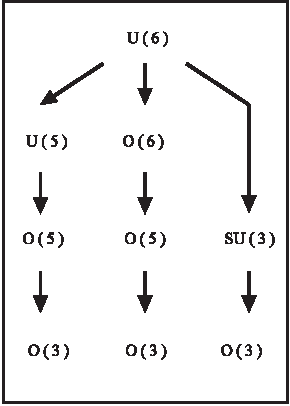
\includegraphics[scale=.65]{figure}
%
% If not, use
%\picplace{5cm}{2cm} % Give the correct figure height and width in cm
%
\caption{If the width of the figure is less than 7.8 cm use the \texttt{sidecapion} command to flush the caption on the left side of the page. If the figure is positioned at the top of the page, align the sidecaption with the top of the figure -- to achieve this you simply need to use the optional argument \texttt{[t]} with the \texttt{sidecaption} command}
\label{fig:1}       % Give a unique label
\end{figure}


\paragraph{Paragraph Heading} %
Instead of simply listing headings of different levels we recommend to let every heading be followed by at least a short passage of text. Furtheron please use the \LaTeX\ automatism for all your cross-references and citations as has already been described in Sect.~\ref{sec:2}.

Please note that the first line of text that follows a heading is not indented, whereas the first lines of all subsequent paragraphs are.

For typesetting numbered lists we recommend to use the \verb|enumerate| environment -- it will automatically render Springer's preferred layout.

\begin{enumerate}
\item{Livelihood and survival mobility are oftentimes coutcomes of uneven socioeconomic development.}
\begin{enumerate}
\item{Livelihood and survival mobility are oftentimes coutcomes of uneven socioeconomic development.}
\item{Livelihood and survival mobility are oftentimes coutcomes of uneven socioeconomic development.}
\end{enumerate}
\item{Livelihood and survival mobility are oftentimes coutcomes of uneven socioeconomic development.}
\end{enumerate}


\subparagraph{Subparagraph Heading} In order to avoid simply listing headings of different levels we recommend to let every heading be followed by at least a short passage of text. Use the \LaTeX\ automatism for all your cross-references and citations as has already been described in Sect.~\ref{sec:2}, see also Fig.~\ref{fig:2}.

Please note that the first line of text that follows a heading is not indented, whereas the first lines of all subsequent paragraphs are.

For unnumbered list we recommend to use the \verb|itemize| environment -- it will automatically render Springer's preferred layout.

\begin{itemize}
\item{Livelihood and survival mobility are oftentimes coutcomes of uneven socioeconomic development, cf. Table~\ref{tab:1}.}
\begin{itemize}
\item{Livelihood and survival mobility are oftentimes coutcomes of uneven socioeconomic development.}
\item{Livelihood and survival mobility are oftentimes coutcomes of uneven socioeconomic development.}
\end{itemize}
\item{Livelihood and survival mobility are oftentimes coutcomes of uneven socioeconomic development.}
\end{itemize}

\begin{figure}[t]
\sidecaption[t]
% Use the relevant command for your figure-insertion program
% to insert the figure file.
% For example, with the option graphics use
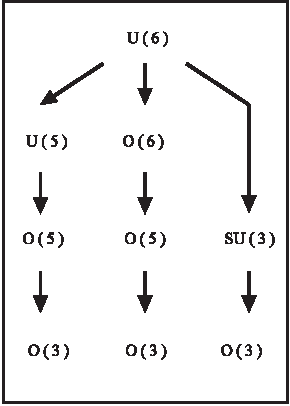
\includegraphics[scale=.65]{figure}
%
% If not, use
%\picplace{5cm}{2cm} % Give the correct figure height and width in cm
%
\caption{Please write your figure caption here}
\label{fig:2}       % Give a unique label
\end{figure}

\runinhead{Run-in Heading Boldface Version} Use the \LaTeX\ automatism for all your cross-references and citations as has already been described in Sect.~\ref{sec:2}.

\subruninhead{Run-in Heading Boldface and Italic Version} Use the \LaTeX\ automatism for all your cross-refer\-ences and citations as has already been described in Sect.~\ref{sec:2}\index{paragraph}.

\subsubruninhead{Run-in Heading Displayed Version} Use the \LaTeX\ automatism for all your cross-refer\-ences and citations as has already been described in Sect.~\ref{sec:2}\index{paragraph}.
% Use the \index{} command to code your index words
%
% For tables use
%
\begin{table}[!t]
\caption{Please write your table caption here}
\label{tab:1}       % Give a unique label
%
% For LaTeX tables use
%
\begin{tabular}{p{2cm}p{2.4cm}p{2cm}p{4.9cm}}
\hline\noalign{\smallskip}
Classes & Subclass & Length & Action Mechanism  \\
\noalign{\smallskip}\svhline\noalign{\smallskip}
Translation & mRNA$^a$  & 22 (19--25) & Translation repression, mRNA cleavage\\
Translation & mRNA cleavage & 21 & mRNA cleavage\\
Translation & mRNA  & 21--22 & mRNA cleavage\\
Translation & mRNA  & 24--26 & Histone and DNA Modification\\
\noalign{\smallskip}\hline\noalign{\smallskip}
\end{tabular}
$^a$ Table foot note (with superscript)
\end{table}
%
\section{Section Heading}
\label{sec:3}
% Always give a unique label
% and use \ref{<label>} for cross-references
% and \cite{<label>} for bibliographic references
% use \sectionmark{}
% to alter or adjust the section heading in the running head
Instead of simply listing headings of different levels we recommend to let every heading be followed by at least a short passage of text. Furtheron please use the \LaTeX\ automatism for all your cross-references and citations as has already been described in Sect.~\ref{sec:2}.

Please note that the first line of text that follows a heading is not indented, whereas the first lines of all subsequent paragraphs are.

If you want to list definitions or the like we recommend to use the Springer-enhanced \verb|description| environment -- it will automatically render Springer's preferred layout.

\begin{description}[Type 1]
\item[Type 1]{That addresses central themes pertainng to migration, health, and disease. In Sect.~\ref{sec:1}, Wilson discusses the role of human migration in infectious disease distributions and patterns.}
\item[Type 2]{That addresses central themes pertainng to migration, health, and disease. In Sect.~\ref{subsec:2}, Wilson discusses the role of human migration in infectious disease distributions and patterns.}
\end{description}

\subsection{Subsection Heading} %
In order to avoid simply listing headings of different levels we recommend to let every heading be followed by at least a short passage of text. Use the \LaTeX\ automatism for all your cross-references and citations citations as has already been described in Sect.~\ref{sec:2}.

Please note that the first line of text that follows a heading is not indented, whereas the first lines of all subsequent paragraphs are.

\begin{svgraybox}
If you want to emphasize complete paragraphs of texts we recommend to use the newly defined Springer class option \verb|graybox| and the newly defined environment \verb|svgraybox|. This will produce a 15 percent screened box 'behind' your text.

If you want to emphasize complete paragraphs of texts we recommend to use the newly defined Springer class option and environment \verb|svgraybox|. This will produce a 15 percent screened box 'behind' your text.
\end{svgraybox}


\subsubsection{Subsubsection Heading}
Instead of simply listing headings of different levels we recommend to let every heading be followed by at least a short passage of text. Furtheron please use the \LaTeX\ automatism for all your cross-references and citations as has already been described in Sect.~\ref{sec:2}.

Please note that the first line of text that follows a heading is not indented, whereas the first lines of all subsequent paragraphs are.

\begin{theorem}
Theorem text goes here.
\end{theorem}
%
% or
%
\begin{definition}
Definition text goes here.
\end{definition}

\begin{proof}
%\smartqed
Proof text goes here.
%\qed
\end{proof}
\begingroup
\renewcommand{\arraystretch}{1.5} % Default value: 1
\begin{table}
	\centering
	\caption{Table template 5}
	\label{t5}
	\begin{tabular}{cc|ccc}
		\noalign{\smallskip}\noalign{\smallskip}\hline\hline
		\multicolumn{2}{c|}{} & A & B & C \\
		\hline
		\multirow{3}{*}{A, C 스침\bigskip} & P 관성계& $T$ & $T$ & $T$ \\
		& Q 관성계& $T$ & $T + \frac{2Lv}{c\sqrt{c^2-v^2}}$ & $T$ \\
		\hline
		\multirow{3}{*}{B, C 스침\bigskip} & P 관성계 & $T+\frac{2L}{v}$ & $T+\frac{2L}{v}$ & $T+\frac{2L\sqrt{c^2-v^2}}{cv}$ \\
		& Q 관성계 & $T+\frac{2L}{v}-\frac{2Lv}{c\sqrt{c^2-v^2}}$ & $T +\frac{2L}{v}$ & $T+\frac{2L\sqrt{c^2-v^2}}{cv}$ \\
		\hline
		\hline
	\end{tabular}
\end{table}
\endgroup

\paragraph{Paragraph Heading} %
Instead of simply listing headings of different levels we recommend to let every heading be followed by at least a short passage of text. Furtheron please use the \LaTeX\ automatism for all your cross-references and citations as has already been described in Sect.~\ref{sec:2}.

Note that the first line of text that follows a heading is not indented, whereas the first lines of all subsequent paragraphs are.
%
% For built-in environments use
%
\begin{theorem}
Theorem text goes here.
\end{theorem}
%
\begin{definition}
Definition text goes here.
\end{definition}
%
\begin{proof}
%\smartqed
Proof text goes here.
%\qed
\end{proof}
%
%
\begin{trailer}{Trailer Head}
If you want to emphasize complete paragraphs of texts in an \verb|Trailer Head| we recommend to
use  \begin{verbatim}\begin{trailer}{Trailer Head}
...
\end{trailer}\end{verbatim}
\end{trailer}
%
\begin{question}{Questions}
If you want to emphasize complete paragraphs of texts in an \verb|Questions| we recommend to
use  \begin{verbatim}\begin{question}{Questions}
...
\end{question}\end{verbatim}
\end{question}
%
%
\begin{important}{Important}
If you want to emphasize complete paragraphs of texts in an \verb|Important| we recommend to
use  \begin{verbatim}\begin{important}{Important}
...
\end{important}\end{verbatim}
\end{important}
%
\clearpage
\begin{warning}{Attention}
If you want to emphasize complete paragraphs of texts in an \verb|Attention| we recommend to
use  \begin{verbatim}\begin{warning}{Attention}
...
\end{warning}\end{verbatim}
\end{warning}

\begin{programcode}{Program Code}
If you want to emphasize complete paragraphs of texts in an \verb|Program Code| we recommend to
use

\verb|\begin{programcode}{Program Code}|

\verb|\begin{verbatim}...\end{verbatim}|

\verb|\end{programcode}|

\end{programcode}
%
\begin{tips}{Tips}
If you want to emphasize complete paragraphs of texts in an \verb|Tips| we recommend to
use  \begin{verbatim}\begin{tips}{Tips}
...
\end{tips}\end{verbatim}
\end{tips}
%
%
\begin{overview}{Overview}
If you want to emphasize complete paragraphs of texts in an \verb|Overview| we recommend to
use  \begin{verbatim}\begin{overview}{Overview}
...
\end{overview}\end{verbatim}
\end{overview}
\clearpage
\begin{backgroundinformation}{Background Information}
If you want to emphasize complete paragraphs of texts in an \verb|Background|
\verb|Information| we recommend to
use

\verb|\begin{backgroundinformation}{Background Information}|

\verb|...|

\verb|\end{backgroundinformation}|
\end{backgroundinformation}
\begin{legaltext}{Legal Text}
If you want to emphasize complete paragraphs of texts in an \verb|Legal Text| we recommend to
use  \begin{verbatim}\begin{legaltext}{Legal Text}
...
\end{legaltext}\end{verbatim}
\end{legaltext}
%
\begin{acknowledgement}
If you want to include acknowledgments of assistance and the like at the end of an individual chapter please use the \verb|acknowledgement| environment -- it will automatically render Springer's preferred layout.
\end{acknowledgement}
%
\section*{Appendix}
\addcontentsline{toc}{section}{Appendix}
%
When placed at the end of a chapter or contribution (as opposed to at the end of the book), the numbering of tables, figures, and equations in the appendix section continues on from that in the main text. Hence please \textit{do not} use the \verb|appendix| command when writing an appendix at the end of your chapter or contribution. If there is only one the appendix is designated ``Appendix'', or ``Appendix 1'', or ``Appendix 2'', etc. if there is more than one.

\begin{equation}
a \times b = c
\end{equation}
% Problems or Exercises should be sorted chapterwise
\section*{Problems}
\addcontentsline{toc}{section}{Problems}
%
% Use the following environment.
% Don't forget to label each problem;
% the label is needed for the solutions' environment
\setcounter{prob}{19}
\setcounter{chapter}{3}
\begin{prob}
\label{prob1}
A given problem or Excercise is described here. The
problem is described here. The problem is described here.
\end{prob}

\begin{prob}
\label{prob2}
\textbf{Problem Heading}\\
(a) The first part of the problem is described here.\\
(b) The second part of the problem is described here.
\end{prob}

\begin{prob}
	\label{prob3}
	\textbf{Generalized tension}\\
	일반적으로 실의 장력을 구하기 위해 가속도를 구하고 이를 이용하여 한 물체에 대한 힘을 분석하지만, 때때로 가속도가 포함되지 않은 식을 이용하는 것이 유용하다.
	
	(a) 그림과 같이 마찰이 없는 수평면에 질량이 각각 $m_{\mathrm{A}}$, $m_\mathrm{B}$인 물체 A, B가 놓여 있고, 각각 반대 방향으로 힘 $F_\mathrm{A}$, $F_\mathrm{B}$가 작용한다. 편의상 물체의 가속도의 방향이 $F_\mathrm{B}$와 같다고 하고, 가속도 $a$를 $m_{\mathrm{A}}$, $m_\mathrm{B}$, $F_\mathrm{A}$, $F_\mathrm{B}$에 대한 식으로 나타내라.\\
	\begin{figure}[H]
		\centering
		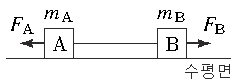
\includegraphics{images/prob.pdf}
	\end{figure}
	(b) 이번에는 A에 작용하는 힘만을 고려하여 실의 장력 $T$를 $m_{\mathrm{A}}$, $F_\mathrm{A}$, $a$에 대한 식으로 나타내라.
	
	(c) 앞선 두 결과를 이용하여 $a$를 소거하여 실의 장력에 대한 식을 얻어라. 그리고 이 식을 기하학적 의미를 해석하라.
	
	(d) \emph{(23학년도 9월 14번)} (가)와 (나)에서 실 q에 걸린 장력을 $m$, $M$, $g$, 빗면 가속도 $a$에 대해 나타내고 두 값이 동일함을 확인하라. (가)에서 실 q에 걸린 장력이 $4mg$임은 명백히 알 수 있다. (가)에서 p가 B를 당기는 힘의 조건이 필요 없음을 확인하라.
	
	(e) \emph{(22학년도 10월 13번)} 물체 A, B에 대해 각각 실에 걸린 장력을 물체와 추의 질량, 중력 가속도 $g$, 빗면 가속도 $a$에 대해 나타내라. 걸린 시간이 4초, 2초인 조건이 필요 없음을 확인하라.
	
\end{prob}
	

%%%%%%%%%%%%%%%%%%%%%%%%% referenc.tex %%%%%%%%%%%%%%%%%%%%%%%%%%%%%%
% sample references
% %
% Use this file as a template for your own input.
%
%%%%%%%%%%%%%%%%%%%%%%%% Springer-Verlag %%%%%%%%%%%%%%%%%%%%%%%%%%
%
% BibTeX users please use
% \bibliographystyle{}
% \bibliography{}
%
\biblstarthook{In view of the parallel print and (chapter-wise) online publication of your book at \url{www.springerlink.com} it has been decided that -- as a genreral rule --  references should be sorted chapter-wise and placed at the end of the individual chapters. However, upon agreement with your contact at Springer you may list your references in a single seperate chapter at the end of your book. Deactivate the class option \texttt{sectrefs} and the \texttt{thebibliography} environment will be put out as a chapter of its own.\\\indent
References may be \textit{cited} in the text either by number (preferred) or by author/year.\footnote{Make sure that all references from the list are cited in the text. Those not cited should be moved to a separate \textit{Further Reading} section or chapter.} If the citatiion in the text is numbered, the reference list should be arranged in ascending order. If the citation in the text is author/year, the reference list should be \textit{sorted} alphabetically and if there are several works by the same author, the following order should be used:
\begin{enumerate}
\item all works by the author alone, ordered chronologically by year of publication
\item all works by the author with a coauthor, ordered alphabetically by coauthor
\item all works by the author with several coauthors, ordered chronologically by year of publication.
\end{enumerate}
The \textit{styling} of references\footnote{Always use the standard abbreviation of a journal's name according to the ISSN \textit{List of Title Word Abbreviations}, see \url{http://www.issn.org/en/node/344}} depends on the subject of your book:
\begin{itemize}
\item The \textit{two} recommended styles for references in books on \textit{mathematical, physical, statistical and computer sciences} are depicted in ~\cite{science-contrib, science-online, science-mono, science-journal, science-DOI} and ~\cite{phys-online, phys-mono, phys-journal, phys-DOI, phys-contrib}.
\item Examples of the most commonly used reference style in books on \textit{Psychology, Social Sciences} are~\cite{psysoc-mono, psysoc-online,psysoc-journal, psysoc-contrib, psysoc-DOI}.
\item Examples for references in books on \textit{Humanities, Linguistics, Philosophy} are~\cite{humlinphil-journal, humlinphil-contrib, humlinphil-mono, humlinphil-online, humlinphil-DOI}.
\item Examples of the basic Springer style used in publications on a wide range of subjects such as \textit{Computer Science, Economics, Engineering, Geosciences, Life Sciences, Medicine, Biomedicine} are ~\cite{basic-contrib, basic-online, basic-journal, basic-DOI, basic-mono}. 
\end{itemize}
}

\begin{thebibliography}{99.}%
% and use \bibitem to create references.
%
% Use the following syntax and markup for your references if 
% the subject of your book is from the field 
% "Mathematics, Physics, Statistics, Computer Science"
%
% Contribution 
\bibitem{science-contrib} Broy, M.: Software engineering --- from auxiliary to key technologies. In: Broy, M., Dener, E. (eds.) Software Pioneers, pp. 10-13. Springer, Heidelberg (2002)
%
% Online Document
\bibitem{science-online} Dod, J.: Effective substances. In: The Dictionary of Substances and Their Effects. Royal Society of Chemistry (1999) Available via DIALOG. \\
\url{http://www.rsc.org/dose/title of subordinate document. Cited 15 Jan 1999}
%
% Monograph
\bibitem{science-mono} Geddes, K.O., Czapor, S.R., Labahn, G.: Algorithms for Computer Algebra. Kluwer, Boston (1992) 
%
% Journal article
\bibitem{science-journal} Hamburger, C.: Quasimonotonicity, regularity and duality for nonlinear systems of partial differential equations. Ann. Mat. Pura. Appl. \textbf{169}, 321--354 (1995)
%
% Journal article by DOI
\bibitem{science-DOI} Slifka, M.K., Whitton, J.L.: Clinical implications of dysregulated cytokine production. J. Mol. Med. (2000) doi: 10.1007/s001090000086 
%
\bigskip

% Use the following (APS) syntax and markup for your references if 
% the subject of your book is from the field 
% "Mathematics, Physics, Statistics, Computer Science"
%
% Online Document
\bibitem{phys-online} J. Dod, in \textit{The Dictionary of Substances and Their Effects}, Royal Society of Chemistry. (Available via DIALOG, 1999), 
\url{http://www.rsc.org/dose/title of subordinate document. Cited 15 Jan 1999}
%
% Monograph
\bibitem{phys-mono} H. Ibach, H. L\"uth, \textit{Solid-State Physics}, 2nd edn. (Springer, New York, 1996), pp. 45-56 
%
% Journal article
\bibitem{phys-journal} S. Preuss, A. Demchuk Jr., M. Stuke, Appl. Phys. A \textbf{61}
%
% Journal article by DOI
\bibitem{phys-DOI} M.K. Slifka, J.L. Whitton, J. Mol. Med., doi: 10.1007/s001090000086
%
% Contribution 
\bibitem{phys-contrib} S.E. Smith, in \textit{Neuromuscular Junction}, ed. by E. Zaimis. Handbook of Experimental Pharmacology, vol 42 (Springer, Heidelberg, 1976), p. 593
%
\bigskip
%
% Use the following syntax and markup for your references if 
% the subject of your book is from the field 
% "Psychology, Social Sciences"
%
%
% Monograph
\bibitem{psysoc-mono} Calfee, R.~C., \& Valencia, R.~R. (1991). \textit{APA guide to preparing manuscripts for journal publication.} Washington, DC: American Psychological Association.
%
% Online Document
\bibitem{psysoc-online} Dod, J. (1999). Effective substances. In: The dictionary of substances and their effects. Royal Society of Chemistry. Available via DIALOG. \\
\url{http://www.rsc.org/dose/Effective substances.} Cited 15 Jan 1999.
%
% Journal article
\bibitem{psysoc-journal} Harris, M., Karper, E., Stacks, G., Hoffman, D., DeNiro, R., Cruz, P., et al. (2001). Writing labs and the Hollywood connection. \textit{J Film} Writing, 44(3), 213--245.
%
% Contribution 
\bibitem{psysoc-contrib} O'Neil, J.~M., \& Egan, J. (1992). Men's and women's gender role journeys: Metaphor for healing, transition, and transformation. In B.~R. Wainrig (Ed.), \textit{Gender issues across the life cycle} (pp. 107--123). New York: Springer.
%
% Journal article by DOI
\bibitem{psysoc-DOI}Kreger, M., Brindis, C.D., Manuel, D.M., Sassoubre, L. (2007). Lessons learned in systems change initiatives: benchmarks and indicators. \textit{American Journal of Community Psychology}, doi: 10.1007/s10464-007-9108-14.
%
%
% Use the following syntax and markup for your references if 
% the subject of your book is from the field 
% "Humanities, Linguistics, Philosophy"
%
\bigskip
%
% Journal article
\bibitem{humlinphil-journal} Alber John, Daniel C. O'Connell, and Sabine Kowal. 2002. Personal perspective in TV interviews. \textit{Pragmatics} 12:257--271
%
% Contribution 
\bibitem{humlinphil-contrib} Cameron, Deborah. 1997. Theoretical debates in feminist linguistics: Questions of sex and gender. In \textit{Gender and discourse}, ed. Ruth Wodak, 99--119. London: Sage Publications.
%
% Monograph
\bibitem{humlinphil-mono} Cameron, Deborah. 1985. \textit{Feminism and linguistic theory.} New York: St. Martin's Press.
%
% Online Document
\bibitem{humlinphil-online} Dod, Jake. 1999. Effective substances. In: The dictionary of substances and their effects. Royal Society of Chemistry. Available via DIALOG. \\
http://www.rsc.org/dose/title of subordinate document. Cited 15 Jan 1999
%
% Journal article by DOI
\bibitem{humlinphil-DOI} Suleiman, Camelia, Daniel C. O'Connell, and Sabine Kowal. 2002. `If you and I, if we, in this later day, lose that sacred fire...': Perspective in political interviews. \textit{Journal of Psycholinguistic Research}. doi: 10.1023/A:1015592129296.
%
%
%
\bigskip
%
%
% Use the following syntax and markup for your references if 
% the subject of your book is from the field 
% "Computer Science, Economics, Engineering, Geosciences, Life Sciences"
%
%
% Contribution 
\bibitem{basic-contrib} Brown B, Aaron M (2001) The politics of nature. In: Smith J (ed) The rise of modern genomics, 3rd edn. Wiley, New York 
%
% Online Document
\bibitem{basic-online} Dod J (1999) Effective Substances. In: The dictionary of substances and their effects. Royal Society of Chemistry. Available via DIALOG. \\
\url{http://www.rsc.org/dose/title of subordinate document. Cited 15 Jan 1999}
%
% Journal article by DOI
\bibitem{basic-DOI} Slifka MK, Whitton JL (2000) Clinical implications of dysregulated cytokine production. J Mol Med, doi: 10.1007/s001090000086
%
% Journal article
\bibitem{basic-journal} Smith J, Jones M Jr, Houghton L et al (1999) Future of health insurance. N Engl J Med 965:325--329
%
% Monograph
\bibitem{basic-mono} South J, Blass B (2001) The future of modern genomics. Blackwell, London 
%
\end{thebibliography}


%%%%%%%%%%%%%%%%%%%%%% chapter.tex %%%%%%%%%%%%%%%%%%%%%%%%%%%%%%%%%
%
% sample chapter
%
% Use this file as a template for your own input.
%
%%%%%%%%%%%%%%%%%%%%%%%% Springer-Verlag %%%%%%%%%%%%%%%%%%%%%%%%%%
%\motto{Use the template \emph{chapter.tex} to style the various elements of your chapter content.}
\chapter{Chapter Heading}
\label{intro} % Always give a unique label
% use \chaptermark{}
% to alter or adjust the chapter heading in the running head

\abstract*{Each chapter should be preceded by an abstract (no more than 200 words) that summarizes the content. The abstract will appear \textit{online} at \url{www.SpringerLink.com} and be available with unrestricted access. This allows unregistered users to read the abstract as a teaser for the complete chapter.
Please use the 'starred' version of the new \texttt{abstract} command for typesetting the text of the online abstracts (cf. source file of this chapter template \texttt{abstract}) and include them with the source files of your manuscript. Use the plain \texttt{abstract} command if the abstract is also to appear in the printed version of the book.}

\abstract{Each chapter should be preceded by an abstract (no more than 200 words) that summarizes the content. The abstract will appear \textit{online} at \url{www.SpringerLink.com} and be available with unrestricted access. This allows unregistered users to read the abstract as a teaser for the complete chapter. \newline\indent
Please use the 'starred' version of the new \texttt{abstract} command for typesetting the text of the online abstracts (cf. source file of this chapter template \texttt{abstract}) and include them with the source files of your manuscript. Use the plain \texttt{abstract} command if the abstract is also to appear in the printed version of the book.}

\section{Section Heading}
\label{sec:1}
Use the template \emph{chapter.tex} together with the document class SVMono (monograph-type books) or SVMult (edited books) to style the various elements of your chapter content conformable to the Springer Nature layout.

\section{Section Heading}
\label{sec:2}
% Always give a unique label
% and use \ref{<label>} for cross-references
% and \cite{<label>} for bibliographic references
% use \sectionmark{}
% to alter or adjust the section heading in the running head
Instead of simply listing headings of different levels we recommend to let every heading be followed by at least a short passage of text. Furtheron please use the \LaTeX\ automatism for all your cross-references and citations.

Please note that the first line of text that follows a heading is not indented, whereas the first lines of all subsequent paragraphs are.

\eject

Use the standard \verb|equation| environment to typeset your equations, e.g.
%
\begin{equation}
a \times b = c\;,
\end{equation}
%
however, for multiline equations we recommend to use the \verb|eqnarray| environment\footnote{In physics texts please activate the class option \texttt{vecphys} to depict your vectors in \textbf{\itshape boldface-italic} type - as is customary for a wide range of physical subjects.}.
\begin{eqnarray}
\left|\nabla U_{\alpha}^{\mu}(y)\right| &\le&\frac1{d-\alpha}\int
\left|\nabla\frac1{|\xi-y|^{d-\alpha}}\right|\,d\mu(\xi) =
\int \frac1{|\xi-y|^{d-\alpha+1}} \,d\mu(\xi)\qquad  \\
&=&(d-\alpha+1) \int\limits_{d(y)}^\infty
\frac{\mu(B(y,r))}{r^{d-\alpha+2}}\,dr \le (d-\alpha+1)
\int\limits_{d(y)}^\infty \frac{r^{d-\alpha}}{r^{d-\alpha+2}}\,dr
\label{eq:01}
\end{eqnarray}

\enlargethispage{24pt}

\subsection{Subsection Heading}
\label{subsec:2}
Instead of simply listing headings of different levels we recommend to let every heading be followed by at least a short passage of text. Further on please use the \LaTeX\ automatism for all your cross-references\index{cross-references} and citations\index{citations} as has already been described in Sect.~\ref{sec:2}.

\begin{quotation}
Please do not use quotation marks when quoting texts! Simply use the \verb|quotation| environment -- it will automatically be rendered in the preferred layout.
\end{quotation}


\subsubsection{Subsubsection Heading}
Instead of simply listing headings of different levels we recommend to let every heading be followed by at least a short passage of text. Furtheron please use the \LaTeX\ automatism for all your cross-references and citations as has already been described in Sect.~\ref{subsec:2}, see also Fig.~\ref{fig:1}\footnote{If you copy text passages, figures, or tables from other works, you must obtain \textit{permission} from the copyright holder (usually the original publisher). Please enclose the signed permission with the manucript. The sources\index{permission to print} must be acknowledged either in the captions, as footnotes or in a separate section of the book.}

Please note that the first line of text that follows a heading is not indented, whereas the first lines of all subsequent paragraphs are.

% For figures use
%
\begin{figure}[b]
\sidecaption
% Use the relevant command for your figure-insertion program
% to insert the figure file.
% For example, with the option graphics use
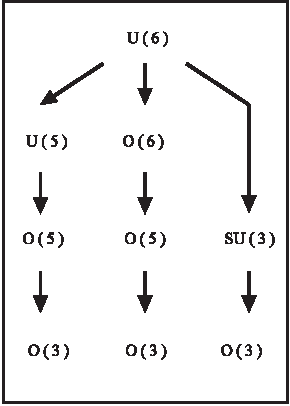
\includegraphics[scale=.65]{figure}
%
% If not, use
%\picplace{5cm}{2cm} % Give the correct figure height and width in cm
%
\caption{If the width of the figure is less than 7.8 cm use the \texttt{sidecapion} command to flush the caption on the left side of the page. If the figure is positioned at the top of the page, align the sidecaption with the top of the figure -- to achieve this you simply need to use the optional argument \texttt{[t]} with the \texttt{sidecaption} command}
\label{fig:1}       % Give a unique label
\end{figure}


\paragraph{Paragraph Heading} %
Instead of simply listing headings of different levels we recommend to let every heading be followed by at least a short passage of text. Furtheron please use the \LaTeX\ automatism for all your cross-references and citations as has already been described in Sect.~\ref{sec:2}.

Please note that the first line of text that follows a heading is not indented, whereas the first lines of all subsequent paragraphs are.

For typesetting numbered lists we recommend to use the \verb|enumerate| environment -- it will automatically render Springer's preferred layout.

\begin{enumerate}
\item{Livelihood and survival mobility are oftentimes coutcomes of uneven socioeconomic development.}
\begin{enumerate}
\item{Livelihood and survival mobility are oftentimes coutcomes of uneven socioeconomic development.}
\item{Livelihood and survival mobility are oftentimes coutcomes of uneven socioeconomic development.}
\end{enumerate}
\item{Livelihood and survival mobility are oftentimes coutcomes of uneven socioeconomic development.}
\end{enumerate}


\subparagraph{Subparagraph Heading} In order to avoid simply listing headings of different levels we recommend to let every heading be followed by at least a short passage of text. Use the \LaTeX\ automatism for all your cross-references and citations as has already been described in Sect.~\ref{sec:2}, see also Fig.~\ref{fig:2}.

Please note that the first line of text that follows a heading is not indented, whereas the first lines of all subsequent paragraphs are.

For unnumbered list we recommend to use the \verb|itemize| environment -- it will automatically render Springer's preferred layout.

\begin{itemize}
\item{Livelihood and survival mobility are oftentimes coutcomes of uneven socioeconomic development, cf. Table~\ref{tab:1}.}
\begin{itemize}
\item{Livelihood and survival mobility are oftentimes coutcomes of uneven socioeconomic development.}
\item{Livelihood and survival mobility are oftentimes coutcomes of uneven socioeconomic development.}
\end{itemize}
\item{Livelihood and survival mobility are oftentimes coutcomes of uneven socioeconomic development.}
\end{itemize}

\begin{figure}[t]
\sidecaption[t]
% Use the relevant command for your figure-insertion program
% to insert the figure file.
% For example, with the option graphics use
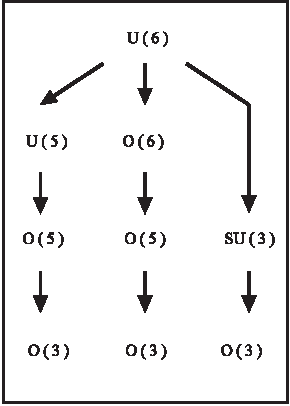
\includegraphics[scale=.65]{figure}
%
% If not, use
%\picplace{5cm}{2cm} % Give the correct figure height and width in cm
%
\caption{Please write your figure caption here}
\label{fig:2}       % Give a unique label
\end{figure}

\runinhead{Run-in Heading Boldface Version} Use the \LaTeX\ automatism for all your cross-references and citations as has already been described in Sect.~\ref{sec:2}.

\subruninhead{Run-in Heading Boldface and Italic Version} Use the \LaTeX\ automatism for all your cross-refer\-ences and citations as has already been described in Sect.~\ref{sec:2}\index{paragraph}.

\subsubruninhead{Run-in Heading Displayed Version} Use the \LaTeX\ automatism for all your cross-refer\-ences and citations as has already been described in Sect.~\ref{sec:2}\index{paragraph}.
% Use the \index{} command to code your index words
%
% For tables use
%
\begin{table}[!t]
\caption{Please write your table caption here}
\label{tab:1}       % Give a unique label
%
% For LaTeX tables use
%
\begin{tabular}{p{2cm}p{2.4cm}p{2cm}p{4.9cm}}
\hline\noalign{\smallskip}
Classes & Subclass & Length & Action Mechanism  \\
\noalign{\smallskip}\svhline\noalign{\smallskip}
Translation & mRNA$^a$  & 22 (19--25) & Translation repression, mRNA cleavage\\
Translation & mRNA cleavage & 21 & mRNA cleavage\\
Translation & mRNA  & 21--22 & mRNA cleavage\\
Translation & mRNA  & 24--26 & Histone and DNA Modification\\
\noalign{\smallskip}\hline\noalign{\smallskip}
\end{tabular}
$^a$ Table foot note (with superscript)
\end{table}
%
\section{Section Heading}
\label{sec:3}
% Always give a unique label
% and use \ref{<label>} for cross-references
% and \cite{<label>} for bibliographic references
% use \sectionmark{}
% to alter or adjust the section heading in the running head
Instead of simply listing headings of different levels we recommend to let every heading be followed by at least a short passage of text. Furtheron please use the \LaTeX\ automatism for all your cross-references and citations as has already been described in Sect.~\ref{sec:2}.

Please note that the first line of text that follows a heading is not indented, whereas the first lines of all subsequent paragraphs are.

If you want to list definitions or the like we recommend to use the Springer-enhanced \verb|description| environment -- it will automatically render Springer's preferred layout.

\begin{description}[Type 1]
\item[Type 1]{That addresses central themes pertainng to migration, health, and disease. In Sect.~\ref{sec:1}, Wilson discusses the role of human migration in infectious disease distributions and patterns.}
\item[Type 2]{That addresses central themes pertainng to migration, health, and disease. In Sect.~\ref{subsec:2}, Wilson discusses the role of human migration in infectious disease distributions and patterns.}
\end{description}

\subsection{Subsection Heading} %
In order to avoid simply listing headings of different levels we recommend to let every heading be followed by at least a short passage of text. Use the \LaTeX\ automatism for all your cross-references and citations citations as has already been described in Sect.~\ref{sec:2}.

Please note that the first line of text that follows a heading is not indented, whereas the first lines of all subsequent paragraphs are.

\begin{svgraybox}
If you want to emphasize complete paragraphs of texts we recommend to use the newly defined Springer class option \verb|graybox| and the newly defined environment \verb|svgraybox|. This will produce a 15 percent screened box 'behind' your text.

If you want to emphasize complete paragraphs of texts we recommend to use the newly defined Springer class option and environment \verb|svgraybox|. This will produce a 15 percent screened box 'behind' your text.
\end{svgraybox}


\subsubsection{Subsubsection Heading}
Instead of simply listing headings of different levels we recommend to let every heading be followed by at least a short passage of text. Furtheron please use the \LaTeX\ automatism for all your cross-references and citations as has already been described in Sect.~\ref{sec:2}.

Please note that the first line of text that follows a heading is not indented, whereas the first lines of all subsequent paragraphs are.

\begin{theorem}
Theorem text goes here.
\end{theorem}
%
% or
%
\begin{definition}
Definition text goes here.
\end{definition}

\begin{proof}
%\smartqed
Proof text goes here.
%\qed
\end{proof}

\paragraph{Paragraph Heading} %
Instead of simply listing headings of different levels we recommend to let every heading be followed by at least a short passage of text. Furtheron please use the \LaTeX\ automatism for all your cross-references and citations as has already been described in Sect.~\ref{sec:2}.

Note that the first line of text that follows a heading is not indented, whereas the first lines of all subsequent paragraphs are.
%
% For built-in environments use
%
\begin{theorem}
Theorem text goes here.
\end{theorem}
%
\begin{definition}
Definition text goes here.
\end{definition}
%
\begin{proof}
%\smartqed
Proof text goes here.
%\qed
\end{proof}
%
%
\begin{trailer}{Trailer Head}
If you want to emphasize complete paragraphs of texts in an \verb|Trailer Head| we recommend to
use  \begin{verbatim}\begin{trailer}{Trailer Head}
...
\end{trailer}\end{verbatim}
\end{trailer}
%
\begin{question}{Questions}
If you want to emphasize complete paragraphs of texts in an \verb|Questions| we recommend to
use  \begin{verbatim}\begin{question}{Questions}
...
\end{question}\end{verbatim}
\end{question}
%
%
\begin{important}{Important}
If you want to emphasize complete paragraphs of texts in an \verb|Important| we recommend to
use  \begin{verbatim}\begin{important}{Important}
...
\end{important}\end{verbatim}
\end{important}
%
\clearpage
\begin{warning}{Attention}
If you want to emphasize complete paragraphs of texts in an \verb|Attention| we recommend to
use  \begin{verbatim}\begin{warning}{Attention}
...
\end{warning}\end{verbatim}
\end{warning}

\begin{programcode}{Program Code}
If you want to emphasize complete paragraphs of texts in an \verb|Program Code| we recommend to
use

\verb|\begin{programcode}{Program Code}|

\verb|\begin{verbatim}...\end{verbatim}|

\verb|\end{programcode}|

\end{programcode}
%
\begin{tips}{Tips}
If you want to emphasize complete paragraphs of texts in an \verb|Tips| we recommend to
use  \begin{verbatim}\begin{tips}{Tips}
...
\end{tips}\end{verbatim}
\end{tips}
%
%
\begin{overview}{Overview}
If you want to emphasize complete paragraphs of texts in an \verb|Overview| we recommend to
use  \begin{verbatim}\begin{overview}{Overview}
...
\end{overview}\end{verbatim}
\end{overview}
\clearpage
\begin{backgroundinformation}{Background Information}
If you want to emphasize complete paragraphs of texts in an \verb|Background|
\verb|Information| we recommend to
use

\verb|\begin{backgroundinformation}{Background Information}|

\verb|...|

\verb|\end{backgroundinformation}|
\end{backgroundinformation}
\begin{legaltext}{Legal Text}
If you want to emphasize complete paragraphs of texts in an \verb|Legal Text| we recommend to
use  \begin{verbatim}\begin{legaltext}{Legal Text}
...
\end{legaltext}\end{verbatim}
\end{legaltext}
%
\begin{acknowledgement}
If you want to include acknowledgments of assistance and the like at the end of an individual chapter please use the \verb|acknowledgement| environment -- it will automatically render Springer's preferred layout.
\end{acknowledgement}
%
\section*{Appendix}
\addcontentsline{toc}{section}{Appendix}
%
When placed at the end of a chapter or contribution (as opposed to at the end of the book), the numbering of tables, figures, and equations in the appendix section continues on from that in the main text. Hence please \textit{do not} use the \verb|appendix| command when writing an appendix at the end of your chapter or contribution. If there is only one the appendix is designated ``Appendix'', or ``Appendix 1'', or ``Appendix 2'', etc. if there is more than one.

\begin{equation}
a \times b = c
\end{equation}
% Problems or Exercises should be sorted chapterwise
\section*{Problems}
\addcontentsline{toc}{section}{Problems}
%
% Use the following environment.
% Don't forget to label each problem;
% the label is needed for the solutions' environment
\begin{prob}
\label{prob1}
A given problem or Excercise is described here. The
problem is described here. The problem is described here.
\end{prob}

\begin{prob}
\label{prob2}
\textbf{Problem Heading}\\
(a) The first part of the problem is described here.\\
(b) The second part of the problem is described here.
\end{prob}

%%%%%%%%%%%%%%%%%%%%%%%% referenc.tex %%%%%%%%%%%%%%%%%%%%%%%%%%%%%%
% sample references
% %
% Use this file as a template for your own input.
%
%%%%%%%%%%%%%%%%%%%%%%%% Springer-Verlag %%%%%%%%%%%%%%%%%%%%%%%%%%
%
% BibTeX users please use
% \bibliographystyle{}
% \bibliography{}
%
\biblstarthook{In view of the parallel print and (chapter-wise) online publication of your book at \url{www.springerlink.com} it has been decided that -- as a genreral rule --  references should be sorted chapter-wise and placed at the end of the individual chapters. However, upon agreement with your contact at Springer you may list your references in a single seperate chapter at the end of your book. Deactivate the class option \texttt{sectrefs} and the \texttt{thebibliography} environment will be put out as a chapter of its own.\\\indent
References may be \textit{cited} in the text either by number (preferred) or by author/year.\footnote{Make sure that all references from the list are cited in the text. Those not cited should be moved to a separate \textit{Further Reading} section or chapter.} If the citatiion in the text is numbered, the reference list should be arranged in ascending order. If the citation in the text is author/year, the reference list should be \textit{sorted} alphabetically and if there are several works by the same author, the following order should be used:
\begin{enumerate}
\item all works by the author alone, ordered chronologically by year of publication
\item all works by the author with a coauthor, ordered alphabetically by coauthor
\item all works by the author with several coauthors, ordered chronologically by year of publication.
\end{enumerate}
The \textit{styling} of references\footnote{Always use the standard abbreviation of a journal's name according to the ISSN \textit{List of Title Word Abbreviations}, see \url{http://www.issn.org/en/node/344}} depends on the subject of your book:
\begin{itemize}
\item The \textit{two} recommended styles for references in books on \textit{mathematical, physical, statistical and computer sciences} are depicted in ~\cite{science-contrib, science-online, science-mono, science-journal, science-DOI} and ~\cite{phys-online, phys-mono, phys-journal, phys-DOI, phys-contrib}.
\item Examples of the most commonly used reference style in books on \textit{Psychology, Social Sciences} are~\cite{psysoc-mono, psysoc-online,psysoc-journal, psysoc-contrib, psysoc-DOI}.
\item Examples for references in books on \textit{Humanities, Linguistics, Philosophy} are~\cite{humlinphil-journal, humlinphil-contrib, humlinphil-mono, humlinphil-online, humlinphil-DOI}.
\item Examples of the basic Springer style used in publications on a wide range of subjects such as \textit{Computer Science, Economics, Engineering, Geosciences, Life Sciences, Medicine, Biomedicine} are ~\cite{basic-contrib, basic-online, basic-journal, basic-DOI, basic-mono}. 
\end{itemize}
}

\begin{thebibliography}{99.}%
% and use \bibitem to create references.
%
% Use the following syntax and markup for your references if 
% the subject of your book is from the field 
% "Mathematics, Physics, Statistics, Computer Science"
%
% Contribution 
\bibitem{science-contrib} Broy, M.: Software engineering --- from auxiliary to key technologies. In: Broy, M., Dener, E. (eds.) Software Pioneers, pp. 10-13. Springer, Heidelberg (2002)
%
% Online Document
\bibitem{science-online} Dod, J.: Effective substances. In: The Dictionary of Substances and Their Effects. Royal Society of Chemistry (1999) Available via DIALOG. \\
\url{http://www.rsc.org/dose/title of subordinate document. Cited 15 Jan 1999}
%
% Monograph
\bibitem{science-mono} Geddes, K.O., Czapor, S.R., Labahn, G.: Algorithms for Computer Algebra. Kluwer, Boston (1992) 
%
% Journal article
\bibitem{science-journal} Hamburger, C.: Quasimonotonicity, regularity and duality for nonlinear systems of partial differential equations. Ann. Mat. Pura. Appl. \textbf{169}, 321--354 (1995)
%
% Journal article by DOI
\bibitem{science-DOI} Slifka, M.K., Whitton, J.L.: Clinical implications of dysregulated cytokine production. J. Mol. Med. (2000) doi: 10.1007/s001090000086 
%
\bigskip

% Use the following (APS) syntax and markup for your references if 
% the subject of your book is from the field 
% "Mathematics, Physics, Statistics, Computer Science"
%
% Online Document
\bibitem{phys-online} J. Dod, in \textit{The Dictionary of Substances and Their Effects}, Royal Society of Chemistry. (Available via DIALOG, 1999), 
\url{http://www.rsc.org/dose/title of subordinate document. Cited 15 Jan 1999}
%
% Monograph
\bibitem{phys-mono} H. Ibach, H. L\"uth, \textit{Solid-State Physics}, 2nd edn. (Springer, New York, 1996), pp. 45-56 
%
% Journal article
\bibitem{phys-journal} S. Preuss, A. Demchuk Jr., M. Stuke, Appl. Phys. A \textbf{61}
%
% Journal article by DOI
\bibitem{phys-DOI} M.K. Slifka, J.L. Whitton, J. Mol. Med., doi: 10.1007/s001090000086
%
% Contribution 
\bibitem{phys-contrib} S.E. Smith, in \textit{Neuromuscular Junction}, ed. by E. Zaimis. Handbook of Experimental Pharmacology, vol 42 (Springer, Heidelberg, 1976), p. 593
%
\bigskip
%
% Use the following syntax and markup for your references if 
% the subject of your book is from the field 
% "Psychology, Social Sciences"
%
%
% Monograph
\bibitem{psysoc-mono} Calfee, R.~C., \& Valencia, R.~R. (1991). \textit{APA guide to preparing manuscripts for journal publication.} Washington, DC: American Psychological Association.
%
% Online Document
\bibitem{psysoc-online} Dod, J. (1999). Effective substances. In: The dictionary of substances and their effects. Royal Society of Chemistry. Available via DIALOG. \\
\url{http://www.rsc.org/dose/Effective substances.} Cited 15 Jan 1999.
%
% Journal article
\bibitem{psysoc-journal} Harris, M., Karper, E., Stacks, G., Hoffman, D., DeNiro, R., Cruz, P., et al. (2001). Writing labs and the Hollywood connection. \textit{J Film} Writing, 44(3), 213--245.
%
% Contribution 
\bibitem{psysoc-contrib} O'Neil, J.~M., \& Egan, J. (1992). Men's and women's gender role journeys: Metaphor for healing, transition, and transformation. In B.~R. Wainrig (Ed.), \textit{Gender issues across the life cycle} (pp. 107--123). New York: Springer.
%
% Journal article by DOI
\bibitem{psysoc-DOI}Kreger, M., Brindis, C.D., Manuel, D.M., Sassoubre, L. (2007). Lessons learned in systems change initiatives: benchmarks and indicators. \textit{American Journal of Community Psychology}, doi: 10.1007/s10464-007-9108-14.
%
%
% Use the following syntax and markup for your references if 
% the subject of your book is from the field 
% "Humanities, Linguistics, Philosophy"
%
\bigskip
%
% Journal article
\bibitem{humlinphil-journal} Alber John, Daniel C. O'Connell, and Sabine Kowal. 2002. Personal perspective in TV interviews. \textit{Pragmatics} 12:257--271
%
% Contribution 
\bibitem{humlinphil-contrib} Cameron, Deborah. 1997. Theoretical debates in feminist linguistics: Questions of sex and gender. In \textit{Gender and discourse}, ed. Ruth Wodak, 99--119. London: Sage Publications.
%
% Monograph
\bibitem{humlinphil-mono} Cameron, Deborah. 1985. \textit{Feminism and linguistic theory.} New York: St. Martin's Press.
%
% Online Document
\bibitem{humlinphil-online} Dod, Jake. 1999. Effective substances. In: The dictionary of substances and their effects. Royal Society of Chemistry. Available via DIALOG. \\
http://www.rsc.org/dose/title of subordinate document. Cited 15 Jan 1999
%
% Journal article by DOI
\bibitem{humlinphil-DOI} Suleiman, Camelia, Daniel C. O'Connell, and Sabine Kowal. 2002. `If you and I, if we, in this later day, lose that sacred fire...': Perspective in political interviews. \textit{Journal of Psycholinguistic Research}. doi: 10.1023/A:1015592129296.
%
%
%
\bigskip
%
%
% Use the following syntax and markup for your references if 
% the subject of your book is from the field 
% "Computer Science, Economics, Engineering, Geosciences, Life Sciences"
%
%
% Contribution 
\bibitem{basic-contrib} Brown B, Aaron M (2001) The politics of nature. In: Smith J (ed) The rise of modern genomics, 3rd edn. Wiley, New York 
%
% Online Document
\bibitem{basic-online} Dod J (1999) Effective Substances. In: The dictionary of substances and their effects. Royal Society of Chemistry. Available via DIALOG. \\
\url{http://www.rsc.org/dose/title of subordinate document. Cited 15 Jan 1999}
%
% Journal article by DOI
\bibitem{basic-DOI} Slifka MK, Whitton JL (2000) Clinical implications of dysregulated cytokine production. J Mol Med, doi: 10.1007/s001090000086
%
% Journal article
\bibitem{basic-journal} Smith J, Jones M Jr, Houghton L et al (1999) Future of health insurance. N Engl J Med 965:325--329
%
% Monograph
\bibitem{basic-mono} South J, Blass B (2001) The future of modern genomics. Blackwell, London 
%
\end{thebibliography}


%%%%%%%%%%%%%%%%%%%%%% appendix.tex %%%%%%%%%%%%%%%%%%%%%%%%%%%%%%%%%
%
% sample appendix
%
% Use this file as a template for your own input.
%
%%%%%%%%%%%%%%%%%%%%%%%% Springer-Verlag %%%%%%%%%%%%%%%%%%%%%%%%%%

\appendix
\motto{All's well that ends well}
\chapter{Chapter Heading}
\label{introA} % Always give a unique label
% use \chaptermark{}
% to alter or adjust the chapter heading in the running head

Use the template \emph{appendix.tex} together with the Springer document class SVMono (monograph-type books) or SVMult (edited books) to style appendix of your book.


\section{Section Heading}
\label{sec:A1}
% Always give a unique label
% and use \ref{<label>} for cross-references
% and \cite{<label>} for bibliographic references
% use \sectionmark{}
% to alter or adjust the section heading in the running head
Instead of simply listing headings of different levels we recommend to let every heading be followed by at least a short passage of text. Furtheron please use the \LaTeX\ automatism for all your cross-references and citations.


\subsection{Subsection Heading}
\label{sec:A2}
Instead of simply listing headings of different levels we recommend to let every heading be followed by at least a short passage of text. Furtheron please use the \LaTeX\ automatism for all your cross-references and citations as has already been described in Sect.~\ref{sec:A1}.

For multiline equations we recommend to use the \verb|eqnarray| environment.
\begin{eqnarray}
\vec{a}\times\vec{b}=\vec{c} \nonumber\\
\vec{a}\times\vec{b}=\vec{c}
\label{eq:A01}
\end{eqnarray}

\subsubsection{Subsubsection Heading}
Instead of simply listing headings of different levels we recommend to let every heading be followed by at least a short passage of text. Furtheron please use the \LaTeX\ automatism for all your cross-references and citations as has already been described in Sect.~\ref{sec:A2}.

Please note that the first line of text that follows a heading is not indented, whereas the first lines of all subsequent paragraphs are.

% For figures use
%
\begin{figure}[t]
\sidecaption[t]
%\centering
% Use the relevant command for your figure-insertion program
% to insert the figure file.
% For example, with the option graphics use
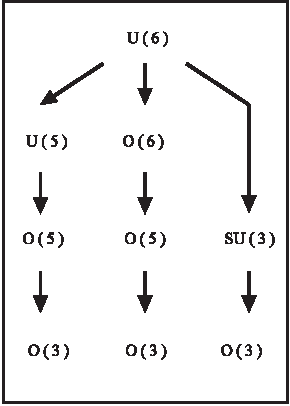
\includegraphics[scale=.65]{figure}
%
% If not, use
%\picplace{5cm}{2cm} % Give the correct figure height and width in cm
%
\caption{Please write your figure caption here}
\label{fig:A1}       % Give a unique label
\end{figure}

% For tables use
%
\begin{table}
\caption{Please write your table caption here}
\label{tab:A1}       % Give a unique label
%
% For LaTeX tables use
%
\begin{tabular}{p{2cm}p{2.4cm}p{2cm}p{4.9cm}}
\hline\noalign{\smallskip}
Classes & Subclass & Length & Action Mechanism  \\
\noalign{\smallskip}\hline\noalign{\smallskip}
Translation & mRNA$^a$  & 22 (19--25) & Translation repression, mRNA cleavage\\
Translation & mRNA cleavage & 21 & mRNA cleavage\\
Translation & mRNA  & 21--22 & mRNA cleavage\\
Translation & mRNA  & 24--26 & Histone and DNA Modification\\
\noalign{\smallskip}\hline\noalign{\smallskip}
\end{tabular}
$^a$ Table foot note (with superscript)
\end{table}
%


\backmatter%%%%%%%%%%%%%%%%%%%%%%%%%%%%%%%%%%%%%%%%%%%%%%%%%%%%%%%
%%%%%%%%%%%%%%%%%%%%%%acronym.tex%%%%%%%%%%%%%%%%%%%%%%%%%%%%%%%%%%%%%%%%%
% sample list of acronyms
%
% Use this file as a template for your own input.
%
%%%%%%%%%%%%%%%%%%%%%%%% Springer %%%%%%%%%%%%%%%%%%%%%%%%%%

\Extrachap{Glossary}


Use the template \emph{glossary.tex} together with the Springer document class SVMono (monograph-type books) or SVMult (edited books) to style your glossary\index{glossary} in the Springer layout.


\runinhead{glossary term} Write here the description of the glossary term. Write here the description of the glossary term. Write here the description of the glossary term.

\runinhead{glossary term} Write here the description of the glossary term. Write here the description of the glossary term. Write here the description of the glossary term.

\runinhead{glossary term} Write here the description of the glossary term. Write here the description of the glossary term. Write here the description of the glossary term.

\runinhead{glossary term} Write here the description of the glossary term. Write here the description of the glossary term. Write here the description of the glossary term.

\runinhead{glossary term} Write here the description of the glossary term. Write here the description of the glossary term. Write here the description of the glossary term.

\Extrachap{Solutions}

\section*{Problems of Chapter~\ref{intro}}

\begin{sol}{prob1}
The solution\index{problems}\index{solutions} is revealed here.
\end{sol}


\begin{sol}{prob2}
\textbf{Problem Heading}\\
(a) The solution of first part is revealed here.\\
(b) The solution of second part is revealed here.
\end{sol}


\printindex

%%%%%%%%%%%%%%%%%%%%%%%%%%%%%%%%%%%%%%%%%%%%%%%%%%%%%%%%%%%%%%%%%%%%%%

\end{document}





